\documentclass[11pt,a4paper,english,oneside]{book}
%\usepackage{etex} %Because of many packages --> Extended TeX.
\usepackage[left=1in, right=1in]{geometry} %Helps to structure the paper layout.
\usepackage[Lenny]{fncychap} %Design of the thesis.
%\usepackage[utf8]{inputenc} %Due to vowels.
\usepackage[T1]{fontenc} % Output font encoding for international characters
\usepackage[english]{babel} %Define the language style.
\usepackage{csquotes}
\usepackage{fancyhdr} %To customize the headers and footers.
\usepackage{appendix} %For the \appendixpage command.
\usepackage{mathtools}
%\usepackage[sort,round]{natbib} %For the bibliography/using biblatex instead.
\usepackage{etoolbox} %To remove the page number on \appendixpage.
\usepackage{setspace} %Use double spacing/using one-half spacing instead.
\usepackage{graphicx,listings,xcolor,textcomp} %For the graphics, listings etc.
\usepackage[margin=10pt, font=small, labelfont=bf, labelsep=endash]{caption}
\usepackage{xparse} %Load for \NewDocumentCommand command.
\usepackage{subcaption}
\usepackage{enumitem} %used to make lists look tidier.
\usepackage{hyperref} %Must be loaded at the end.
\usepackage{cleveref} %For the command \cref, load after hyperref.
\usepackage{makecell} %To make nice tables

% :::~ This is the configuration for the bibliography. DO NOT CHANGE
\usepackage[
backend=biber,
style=authoryear,
natbib=false,
maxcitenames=2,
minbibnames=1, maxbibnames=99, 
url=false, 
doi=true,
]{biblatex}

\addbibresource{thesis.bib}

\setlength{\parindent}{0pt}
%\bibliographystyle{abbrvnat} %Reference style.

\definecolor{uzh@darkblue}{RGB}{5,85,158}
\definecolor{uzh@blue}{RGB}{0,39,163}
\definecolor{uzh@lightblue}{RGB}{167,180,217}
\definecolor{uzh@grey}{RGB}{163,173,183}
\definecolor{uzh@lightgrey}{RGB}{212,219,224}
\definecolor{uzh@darkgrey}{RGB}{151,165,175}
\definecolor{uzh@red}{RGB}{220,96,39}
\definecolor{uzh@darkred}{RGB}{216,88,52}
\definecolor{uzh@lightred}{RGB}{240,193,166}
\definecolor{uzh@green}{RGB}{136,215,49}
\definecolor{uzh@darkgreen}{RGB}{123,171,65}
\definecolor{uzh@lightgreen}{RGB}{201,231,161}
% 

%Setup of the reference links.
\hypersetup{
     colorlinks=true,
     linkcolor=uzh@blue,
     citecolor=uzh@blue,
     filecolor=uzh@red,
     urlcolor=uzh@red}



\usepackage{fontspec}


\setmainfont{Arial}
%Define some reasonable margins.
\setlength{\textwidth}{6.6in}
\setlength{\textheight}{8.8in}
\setlength{\topmargin}{-0.1in}
\setlength{\oddsidemargin}{0in}
\setlength{\parskip}{1mm}


\usepackage{sectsty}
%\allsectionsfont{\color{blue}\itshape\underline}
\sectionfont{\color{uzh@blue}}
\subsectionfont{\color{uzh@darkblue}}
\paragraphfont{\color{uzh@darkblue}}

%New command for the UZH logo.
\newcommand*{\uzhlogo}{
\includegraphics[height=2cm]{Logo-UZH-black}}
\newcommand*{\bcclogo}{
\includegraphics[height=2.2cm]{Logo-BCC-black}}
\newcommand*{\bdltlogo}{
\includegraphics[height=2cm]{Logo-BDLT-black}}

%New command for the differential d to have an ordinary d.
\makeatletter
  \newcommand{\ud}{\mathrm{d}}
\makeatother

%Remove page number on \appendixpage. Use the package 'etoolbox'.
\makeatletter
\patchcmd{\@chap@pppage}{\thispagestyle{plain}}{\thispagestyle{empty}}{}{}
\makeatother

%----------------------------------------------------------------------------------------
%	TITLE PAGE
%----------------------------------------------------------------------------------------
\newcommand*{\titleGP}{\begingroup %Create the command for including the title page in the document.
\centering %Center all text.
\vspace*{\baselineskip} %White space at the top of the page.
\uzhlogo\hspace{8cm}\bcclogo\\[2\baselineskip] %University Logo.

\rule{\textwidth}{1.6pt}\vspace*{-\baselineskip}\vspace*{2pt} %Thick horizontal line.
\rule{\textwidth}{0.4pt}\\[\baselineskip] %Thin horizontal line.
{\LARGE \sc Analysis of Implementing a Smart Contract in Weather Insurance using Chainlink Oracles}\\[0.2\baselineskip] %Title.
\rule{\textwidth}{0.4pt}\vspace*{-\baselineskip}\vspace{3.2pt} %Thin horizontal line.
\rule{\textwidth}{1.6pt}\\[2\baselineskip] %Thick horizontal line.
\scshape %Small caps.
Bachelor Thesis\\[2\baselineskip]
Submitted in partial fulfillment of the requirements for \\ the degree of Bachelor of Science \par
\vspace*{2\baselineskip}
Author\\
{\Large \textbf{Aeberhard Elia Andreas} \\ [8pt]
 }
Gmeindhusplatz 4 \\ 5223 Riniken \\[5pt]
Matriculation Number: \textbf{19-925-957}\\[8pt]
 Email: \texttt{ \href{mailto:elia.aeberhard@uzh.ch} {elia.aeberhard@uzh.ch} }  \\


\vspace*{2\baselineskip}
Supervisor\\
{\Large Prof. Dr Claudio J. Tessone\\[8pt]
\small Blockchain \& Distributed Ledger Technologies\\[5pt]Department of Informatics \\[8pt]University of Zurich\par}
\vspace*{2\baselineskip}

\vfill
{\scshape Date of Submission: [ Date ]} \\[0.3\baselineskip]
\endgroup}

%Special header and footer style for the executive summary and Task Assignment section.
\fancypagestyle{firststyle}{%
  \fancyhf{}%
  \renewcommand{\headrulewidth}{0pt}
  \fancyfoot[C]{\thepage}}

%Customize headers and footers.
\pagestyle{fancy}
\fancyhead[R]{\thepage}
\fancyhead[L]{\rightmark}
\fancyfoot[L]{Elia Aeberhard}
\fancyfoot[C]{}
\fancyfoot[R]{Bachelor Thesis}

%Define the signature line with dots.
\NewDocumentCommand \dotbox {o O{.5\linewidth} m O{3ex} O{\linewidth}}
{
  \begin{minipage}{7cm}
    \makebox[7cm][l]{\,.\dotfill}
    \\
    \makebox[7cm][l]{\,#3}
  \end{minipage}
}

\begin{document}
\thispagestyle{empty}
\titleGP
\newpage
\onehalfspacing
\setcounter{page}{1}
\pagenumbering{Roman}

\section*{Executive Summary}
\thispagestyle{firststyle}
Write  this  last.   It  is  an  overview  of  your  whole  thesis,  and  is  between  200-300words.. . .


\tableofcontents
\listoffigures
\listoftables
\newpage
\pagenumbering{arabic}

\chapter{Introduction}\label{chapter:introduction} 
Weather-related disasters are among the most significant challenges of the 21st century. Their frequency and severity continue to increase steadily due to climate change, causing destruction and substantial economic losses for individuals, businesses and governments. Insurance has long been the primary tool to reduce the financial impact of such disasters, providing a safety net that promotes stability. However, traditional insurance is increasingly struggling to address the scale and complexity of modern and future climate risks, which are expected to increase due to greenhouse gas emissions \autocites{van2006impacts}{monasterolo2020climate}{jones2005assessing}.

Traditional weather insurance systems struggle with inefficiencies such as manual claim assessments, systemic risk and a lack of transparency and trust, which highlight the limitations of these systems and underscore the need for innovative solutions to address the growing modern and future climate risks. By leveraging key features such as decentralization, transparency and automation, a blockchain-based weather insurance system is able to overcome the inefficiencies of traditional models \autocites{Salem2021Developing}{Omar2023Blockchain-Based}. This thesis aims to address the limitations of traditional models in modern and future climate risks by utilizing key features of blockchain technology in a prototype and evaluates its feasibility in practical applications such as the renewable energy sector and disaster relief efforts.

\section{Background}\label{section:background}
In 2016, global disasters accounted for USD 175 billion in economic losses. USD 54 billion of these losses were insured, resulting in uninsured losses of USD 121 billion \autocite{swissre2017}. These losses highlight the importance of weather insurance in providing financial protection for individuals, businesses and governments. However, the significant gap between insured and uninsured losses highlights the insufficiency of current insurance solutions in addressing the scope of climate-related risks. For comparison, international humanitarian assistance reached USD 28 billion in 2015, making the uninsured losses of 2016 over four times that amount \autocite{development2016humanitarian}.

Predictions suggest a worsening of these losses due to intensifying climate risks. Insurance premiums are projected to increase by more than 5 percent and property losses from natural disasters could rise by up to 60 percent by 2040. These escalating costs reflect the growing frequency and severity of extreme weather events, including hurricanes, floods, droughts and wildfires. This increased probability of extreme weather events is also expected to lead to higher weather insurance premiums, highlighting the significant challenges posed by intensifying climate risks \autocites{cho2022climate}{tucker1997climate}.

\subsection{Existing Weather Insurance}
Traditional weather insurance primarily consisted of crop insurance. The policy in this type of contract was typically conducted bilaterally between an individual or business and the insurance company. If a loss occurred on the crop of the individual or business due to weather conditions, an assessment had to be done by the insurance company and the insurance payout sum was determined based on the specific circumstances \autocite{michler2022risk}.

Crop insurance has several major problems associated with it. One of these problems is the manual process of analyzing and determining the loss in monetary terms by an insurance company representative. Other problems include systemic risk, where many insurance holders in the same region are at risk of being affected by extreme weather conditions simultaneously and asymmetric information, where insurance holders behave more riskily than they normally would because they know they are insured \autocite{makki2002crop}.

\sloppy A more modern approach to weather insurance, compared to traditional crop insurance, is weather-based index insurance. The key difference is that weather-based index insurance relies on a measurable variable (such as a temperature drop below a certain threshold or a specific amount of rainfall) and the underlying weather data is provided by a reference weather station. The goal is for the criteria (e.g., the temperature threshold) to reflect the financial loss experienced by the insurance holder, such as the loss of a cornfield due to adverse weather conditions \autocite{kajwang2022weather}.

\subsection{Key Limitations in Existing Weather Insurance}\label{section:key_limitations_existing_insurance}
Despite the advancements in traditional weather insurance, several challenges continue to reduce its effectiveness and accessibility. The following subsections explore these challenges and elaborate on how blockchain technology can be used in a weather insurance system to address them.

\subsubsection{Administrative Costs}
In traditional crop insurance, administrative costs make up 35\% to 40\% of the insurance outlays, while the remaining portion goes toward other costs such as the insurance payout and reinsurance costs \autocite{glauber2004crop}. The majority of these administrative costs consist of loss assessment, monitoring, claims and underwriting expenses.
 
In index insurance, administrative costs are significantly lower than in crop insurance because the payouts are based on predefined weather indices rather than assessing individual losses. This index-based insurance model also reduces moral hazards since the payouts are triggered by weather events rather than individual actions. \textcite{kusuma2018viable} propose a weather-based index insurance for rice in Indonesia. It is designed to be cost-effective by basing the insured amount on the cost of inputs (e.g., seed and fertilizer) rather than covering individual revenue losses.
 
In \cref{section:smart_contracts_insurance}, this thesis will discuss how smart contracts can be used to lower administrative costs through automated processes even further than weather-based index insurance.
 
\subsubsection{Systemic Risk}\label{systemic_risk}
A key limitation of existing weather insurance is the systemic risk it poses. \textcite{xu2010systemic} explain how weather risk is systemic in nature, meaning that weather-related events like droughts or floods often affect entire regions rather than isolated areas. In such events, a large number of insurance holders would file claims simultaneously, making it difficult for the insurance company to pay out all these claims at the same time. The study further shows that systemic risk is one of the key reasons why existing weather-based insurance markets have struggled and often require government subsidies, especially in the case of crop insurance. This thesis will examine how a blockchain-based weather insurance solution could further reduce systemic risk by creating more decentralized risk pools.
 
\subsubsection{Lack of Transparency and Trust}
The reliance of the insurance industry on trust is well established \autocite{courbage2021trust}. Trust plays a key role in fostering collaboration between insurance providers and policyholders, ensuring a smooth execution of transactions and minimizing disputes. \textcite{guiso2012trust} further finds that in low-trust environments, transaction costs and subsequently, insurance premiums are unusually high. For example, \textcite{gennaioli2022trust} found that in countries with a low trust index in financial markets, the percentage of rejected claims can rise to as much as 35\%, while globally, the average hovers around 20\%. These statistics underline the importance of maintaining high levels of trust to promote activity, cost-effectiveness and fairness in insurance systems.

Due to the immutability and public nature of blockchain, it offers a trustworthy foundation by preventing fraudulent activities such as altering transactions, falsifying claims or tampering with data \autocite{Ahmad2024Fraud}. Transactions recorded on the blockchain are tamper-proof and stored transparently across a worldwide network of nodes, through which all participants can independently verify the relevant information \autocite{eigelshoven2021cryptocurrency}. However, \textcite{hawlitschek2018limits} note that completely trust-free systems may not be possible, as they may still rely on trusted intermediaries, particularly for off-chain data integration. By providing fraudulent data, intermediaries can compromise the entire system, as a smart contract running on the blockchain cannot validate external data. In our system, we will also use intermediary entities, such as Chainlink and Google Cloud Platform (GCP) Datasets (see \cref{section:prototype_development}). While these intermediaries introduce potential vulnerabilities, we will discuss later in the thesis how to mitigate such vulnerabilities to ensure a trustworthy system \autocite{Khan2022Investigation}.

\subsection{Oracles}
Blockchain oracles serve as intermediaries between on-chain smart contracts and off-chain data sources and enable smart contracts to access and use real-world information \autocite{caldarelli2022overview}. By fetching, verifying and transmitting external data to the blockchain, oracles allow smart contracts to make decisions and execute their logic based on up-to-date information \autocite{pasdar2023connect}. In this thesis, we will utilize such oracles to integrate real-world weather data into a blockchain-based weather insurance system.

\section{Smart Contracts in Insurance}\label{section:smart_contracts_insurance}
Smart contracts are emerging as an innovative technology in the insurance industry, offering the potential to automate processes, enhance transparency and improve trust among its users. In this section, we explore two notable examples: AXA's Fizzy and Lemonade. These case studies highlight the potential of blockchain-based solutions and their real-world applicability.

\subsection{Early Applications: Fizzy and Lemonade}
In 2017, the insurance company AXA launched Fizzy, a flight insurance product based on smart contract technology. It was one of the earliest examples of the adoption of blockchain technology in the insurance industry. Fizzy was quite simple: a customer entered their flight details and paid a premium for the insurance. Later, Fizzy used an oracle to check wether the flight had been delayed by more than two hours and, if so, automatically triggered a payment \autocite{hoffmann2021double}.

Another example is Lemonade, a pioneering company in the InsuranceTech industry. It uses a combination of artificial intelligence and smart contracts to identify, analyze and streamline claims processes automatically. A customer can buy a policy via Lemonade's app, where the smart contract defines and enforces the terms of the coverage. When an insured event, such as theft or damage, occurs, the customer can file a claim directly through the app. Lemonade's AI then immediately reviews the claim, validates the circumstances and triggers the smart contract to execute the payout. This process is seamless and transparent and can be completed within minutes, in contrast to the lengthy and often cumbersome claim handling of traditional insurance, where multiple intermediaries, approvals and other entities are involved. \autocites{la2023insurtech}{tardieu2020case}.

\section{Technical and Regulatory Challenges of Smart Contracts}\label{section:regulatory_technical_challenges}
\textcite{gatteschi2018blockchain} express concerns that blockchain technology, including smart contracts, is still being explored and not yet ready for its benefits to become more evident. While the technology offers significant advantages, its adoption in industries like insurance is often hindered by technical and regulatory challenges.

\subsection{Technical Challenges}\label{technical_challenges_chapter1}
In the insurance industry, a significant challenge is the technical readiness of smart contracts. These contracts depend on oracles, external data sources that provide real-world information necessary for their operations. Oracles serve as the bridge between off-chain and on-chain data, delivering critical inputs such as weather data, flight delays or other metrics relevant to insurance claims. The reliability of a smart contract depends on the accuracy and integrity of the data provided by these oracles, which are essential to the system. However, oracles can also introduce vulnerabilities, such as data corruption or tampering, which undermine the trustworthiness of the system \autocites{Sheldon2020Auditing}{Al-Breiki2020Trustworthy}.

Apart from oracle vulnerabilities, there are also concerns about the scalability of smart contracts, especially on the Ethereum blockchain. With a high volume of data and transactions, the performance of the system can degrade due to computational and storage limitations. The Ethereum blockchain often faces challenges with transaction throughput, latency and high gas fees, which reduce the potential for implementing a blockchain-based insurance system at scale \autocites{Khan2021Systematic}{Chauhan2018Blockchain}.

Other technical issues include the lack of standardization in the development and implementation of smart contracts and the fact that their code is vulnerable to bugs that can be exploited by malicious actors. The immutability of a smart contract once deployed on the blockchain underscores the need for extensive testing, auditing and monitoring to ensure the security of a blockchain-based insurance system \autocite{Chen2019Defining}.

\subsection{Regulatory Challenges}\label{regulatory_challenges_chapter1}
Another important point to consider is the variety of regulatory issues associated with smart contracts. These challenges originate from inconsistencies in legal definitions, concerns about consumer protection, compliance requirements and the complexities of cross-border transactions. In this section, we will explore these regulatory issues and describe how they may impact the adoption and functionality of blockchain-based insurance systems.

\subsubsection{Smart Contract as Legally Binding Agreements}
There is no universally accepted definition of a smart contract, which creates difficulties in establishing their legal status across different jurisdictions. While some jurisdictions may recognize smart contracts as legally binding agreements, others may not, leading to ambiguity for businesses and individuals operating across multiple legal systems. This lack of standardization complicates the enforceability of smart contracts and may create additional legal complications for the users and providers of such systems \autocite{Mik2017Smart}.

\subsubsection{Consumer Protection Laws}
Additionally, consumer protection laws pose challenges for the adoption of smart contracts. Automated transactions initiated by smart contracts may violate local regulations if consumers lack the ability to contest or reverse them. For example, a customer could encounter issues with a smart contract that automatically executes a payment, even in situations where the transaction is disputed or unintended. This lack of reversibility could lead to legal disputes and undermine trust in the system \autocite{ferreira2021regulating}.

\subsubsection{Compliance with Data Privacy}
Another critical concern is compliance with data privacy regulations, such as the General Data Protection Regulation (GDPR) in the European Union. Smart contracts often store data on an immutable blockchain, which could conflict with legal requirements, such as the "right to be forgotten" \autocite{mantelero2013eu}. This creates significant challenges for developers and operators of blockchain-based systems, as meeting the demands of immutability and data privacy simultaneously can be difficult. Ensuring that sensitive user data is not exposed or permanently stored may not be possible for certain implementations or use cases of a blockchain-based system.

\subsubsection{Cross Border Disputes}
The cross-border nature of blockchain networks and smart contracts introduces additional complexities, as transactions and data exchanges often involve components and systems located in different countries, each with its own regulatory framework. Policies such as taxation, anti-money laundering (AML) compliance and know-your-customer (KYC) requirements make it challenging for the provider of a blockchain-based system to navigate and address these legal issues effectively \autocites{Spafford2019Blockchain}{Li2023Cross-Border}.

\section{Objectives}\label{section:objectives}
Even though the weather-based index insurance approach represents a significant improvement over traditional crop insurance, there are still many problems associated with it (see \cref{section:key_limitations_existing_insurance}). These limitations reduce accessibility, efficiency and the range of weather insurance solutions available to individuals and businesses, especially in developing areas. The key objective of this thesis is to develop blockchain-based weather insurance prototype that addresses the challenges and drawbacks of traditional insurance models and identify its potential applications as well as its limitations. The specific objectives are as follows:

\begin{itemize}
    \item Identify and analyze the key challenges of current weather insurance solutions.
    \item Propose a blockchain-based weather insurance design that utilizes decentralized oracles and globally available weather data.
    \item Compare the blockchain-based solution to traditional weather insurance solutions in order to assess its potential and identify improvements in terms of efficiency, transparency and trust.
    \item Analyze potential real-world applications of a blockchain-based system and discuss its limitations
\end{itemize}
\chapter{Methodology}\label{chapter:methodology}
\section{Research Design}\label{section:research_design}
\section{Data Collection}\label{section:data_collection}
\section{Prototype development}\label{section:prototype_development}
\chapter{Development of the Prototype}\label{chapter:development_prototype}
This chapter outlines the development of a blockchain-based weather insurance prototype with a focus on the design, architecture and functionality. First, we present the necessary requirements for the system, which include functional, non-functional and technical aspects. Later, the architecture of the proposed system is introduced, which provide an overview of the key components of the system, including smart contracts, Chainlink oracles and Google Cloud Public Datasets.

The data flow section describes how the different components of the system work together to enable purchasing policies, executing eligibility checks and paying out claims. Finally, real-world applications of the system are explored, which demonstrate how the prototype can address specific challenges across diverse sectors and industries, such as disaster relief, tourism and renewable energy.

The chapter establishes the foundation for evaluating the proposed solution, highlighting its potential and limitations in terms of transparency, efficiency and trust compared to traditional insurance systems.

\section{Requirements}\label{section:requirements}
In order to provide the blockchain-based weather insurance, our system must fulfill several key requirements. In this section we describe each category of requirements in a dedicated subsection. These requirements are derived from the objectives outlined in \cref{section:objectives} and are designed to address the limitations of traditional models described in \cref{section:key_limitations_existing_insurance}.

\subsection{Functional Requirements}\label{subsection:functionalRequirements}
\begin{itemize}
    \item \textbf{User Interaction}
    \begin{itemize}
        \item The system must provide a user interface for purchasing policies and triggering payout eligibility checks. 
    \end{itemize}

    \item \textbf{Weather Data Integration} 
    \begin{itemize}
        \item The system must be able to receive and process global weather data from reliable and trusted external sources such as Global Surface Summary of the Day (GSOD) and Global Forecast System (GFS).
        \item The weather data must be validated using a decentralized mechanism to ensure reliability and prevent single points of failure.
    \end{itemize}
    
    \item \textbf{Smart Contract}
    \begin{itemize}
        \item The smart contract must allow end users to purchase and terminate weather-based insurance policies based on parameters provided by the end user and the external sources.
        \item The smart contract must store the policy terms.
        \item The smart contract must be able to perform eligibility checks on existing policies.
        \item The smart contract must be able to payout funds for policies that have passed eligibility checks.
    \end{itemize}
    
    \item \textbf{Oracle Integration}
    \begin{itemize}
        \item The system must use Chainlink oracles to retrieve and verify weather data from GCP datasets.
    \end{itemize}
\end{itemize}

\subsection{Non-Functional Requirements}
\begin{enumerate}
    \item \textbf{Security}
    \begin{itemize}
        \item All the bilateral interactions between the smart contract, Chainlink oracles, GCP and the end user must be secure.
    \end{itemize}
    
    \item \textbf{Scalability}
    \begin{itemize}
        \item The system must be able to scale to handle large amounts of policies and end users.
    \end{itemize}
    
    \item \textbf{Transparency}
    \begin{itemize}
        \item All transactions and insurance claims must be recorded on the blockchain for transparency purposes.
    \end{itemize}
\end{enumerate}

\subsection{Technical Requirements}\label{subsection:technicalRequirements}
\begin{enumerate}
    \item \textbf{Blockchain Platform}
    \begin{itemize}
        \item The smart contract must be deployed on the Ethereum blockchain.
    \end{itemize}
    
    \item \textbf{Data Retrieval}
    \begin{itemize}
        \item The system must be able to retrieve weather data from GCP.
    \end{itemize}
    
    \item \textbf{Chainlink Oracle}
    \begin{itemize}
        \item The system must integrate with a Chainlink node to facilitate data retrieval from GCP.
    \end{itemize}
\end{enumerate}

\section{Architecture}
In this section, we outline the architecture of our blockchain-based weather insurance system. We begin with a high-level overview of the system, followed by detailed subsections that focus on the key components and their roles within the architecture.

\subsection{General Overview}\label{subsection:generalOverview}
In \cref{fig:generalArchitecture} we present an overview of the general architecture of our proposed system. The center of the architecture is the smart contract deployed on the Ethereum blockchain. It manages all policies and handles the payout process. The end user interacts directly with the smart contract through the use of a decentralized app (see \cref{subsection:decentralizedApp}), where they can request insurance policies and eligibility checks.

The weather data is provided by Global Surface Summary of the Day (GSOD) and Global Forecast System (GFS), respectively. These datasets can be accessed via GCP BigQuery and GCP Storage through the GCP API interface. To bridge the gap between the off-chain data from GCP and the on-chain smart contract, the system uses a Chainlink oracle (see \cref{subsection:ChainlinkOracle}). This Chainlink oracle retrieves the weather data from GCP through its API interface and passes it on to the smart contract on the Ethereum blockchain.

\begin{figure}[ht]
    \centering
    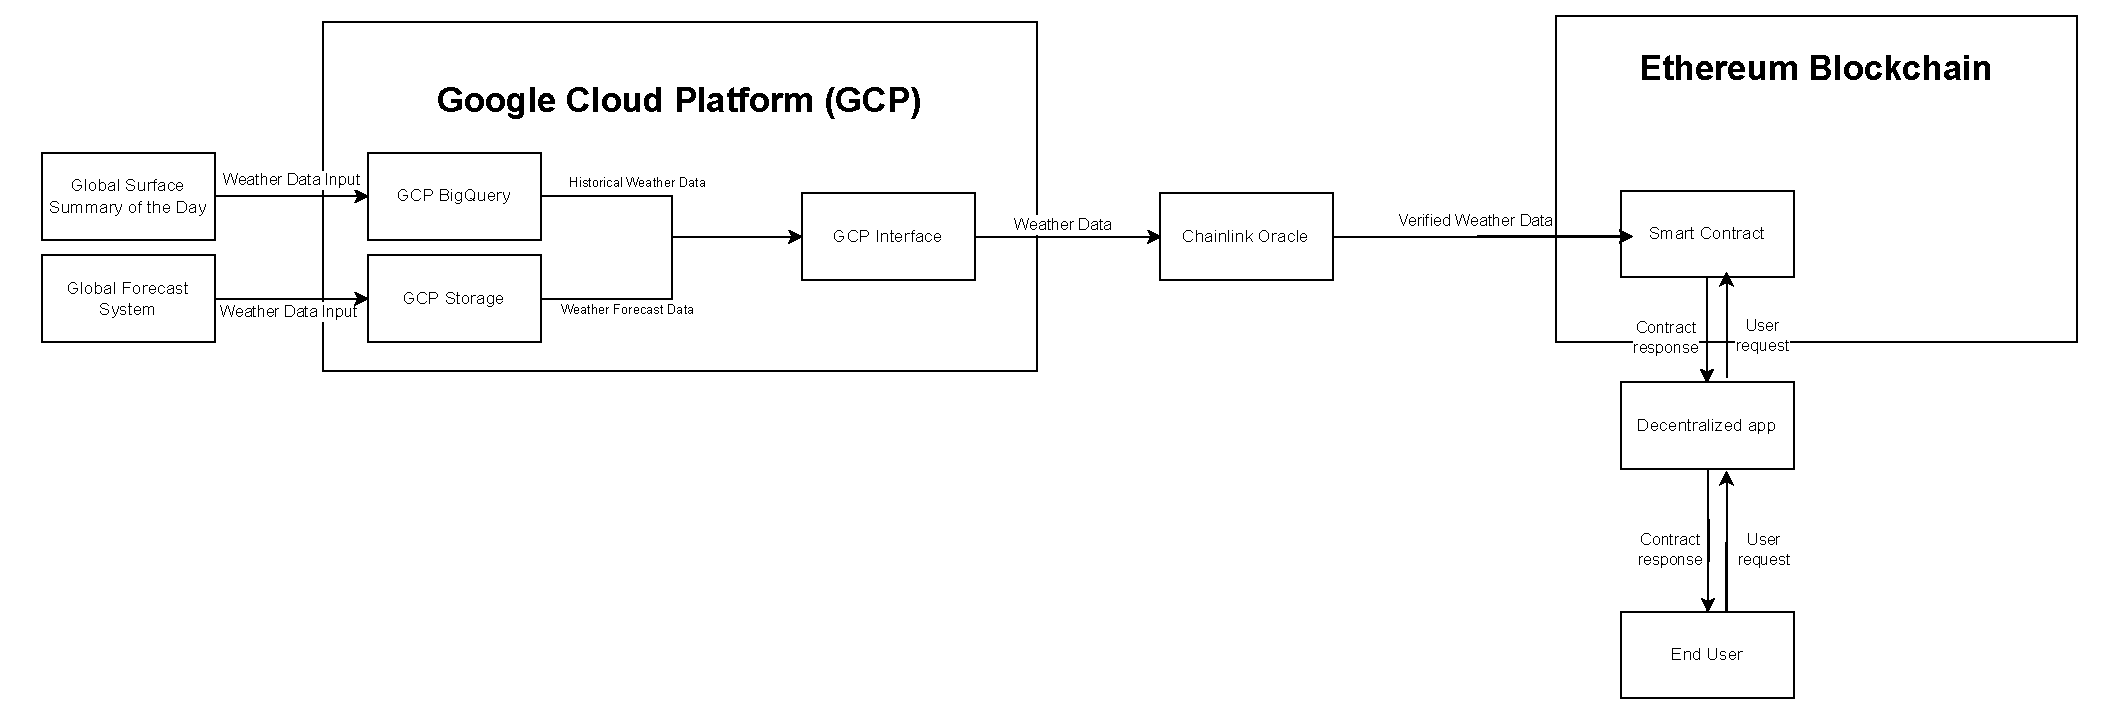
\includegraphics[width=1\textwidth]{figures/architecture-overview.drawio.pdf}
    \caption{High-level architectural diagram of the proposed blockchain-based weather insurance system, illustrating interactions between the smart contract, decentralized app, Chainlink and Google Cloud Public Datasets. \textit{Source: Author's own representation.}}
    \label{fig:generalArchitecture}
\end{figure}

This architecture effectively addresses the technical requirements defined in \cref{subsection:technicalRequirements} and ensures compatible and reliable communications between each component.

\subsection{Decentralized App}\label{subsection:decentralizedApp}
The decentralized application (DApp) allows a non-technical end user to directly interact with the blockchain. Through its interface, a user can request insurance policies, eligibility checks and receive payout funds. Unlike traditional applications, which interact with a centrally managed backend, decentralized applications interact directly with a decentralized blockchain network.

This interaction requires a digital wallet (for example, MetaMask), which enables the user to initiate and sign a transaction when making a request, such as purchasing an insurance policy. In our architecture, the dApp serves as the primary interface in order for the end-users to interact with the smart contract. 

\subsection{Integration of Chainlink Oracles and the Google Cloud Platform}\label{subsection:ChainlinkOracle}
Since the weather data from GSOD and GFS, which is accessed through the GCP datasets, is not directly available from the on-chain environment of the smart contract, we need to leverage oracles, which retrieve and verify external data before delivering it to the blockchain.

In our proposed system, Chainlink oracles are used to securely interact with the GCP and pass the data on to the smart contract. The Chainlink oracle network consists of globally distributed nodes. When a request is triggered, multiple nodes independently access GCP and receive the weather data specified in the request. If any nodes return results that differ from the majority, they are flagged as potentially malicious. This decentralized approach ensures that only verified and reliable weather data is passed on to the smart contract.

\section{Data Flow}
In this section, we examine the two primary data flow scenarios central to our blockchain-based weather insurance system: the process of purchasing a weather insurance policy (see \cref{subsection:purchasePolicyFlow}) and the process of triggering a policy payout (see \cref{subsection:policyPayoutTrigger}). These scenarios represent the fundamental interactions between the end user, the smart contract and the external data sources. In the subsequent chapters, we elaborate on the core functionalities utilized in the two scenarios, such as the process of retrieving weather data and calculating the policy conditions.

\subsection{Purchase Weather Insurance Policy}\label{subsection:purchasePolicyFlow}
The sequence diagram in \cref{fig:purchasePolicyFlow} outlines the steps involved in purchasing a weather insurance policy in our proposed system. The main components are the end user, the smart contract, Chainlink oracles and the Google Cloud Platform (GCP). Each of these components plays a central role in enabling the policy purchase and the associated data retrieval and validation processes. Each request between components includes a set of parameters. These parameters contain the necessary information that each component needs in order to perform its role and functions accurately. For example, in a purchase policy request, parameters such as location, coverage duration and type of coverage are sent to the smart contract. Table \cref{tab:flowRequests} contains all requests with their respective parameters.

\begin{figure}[ht]
    \centering
    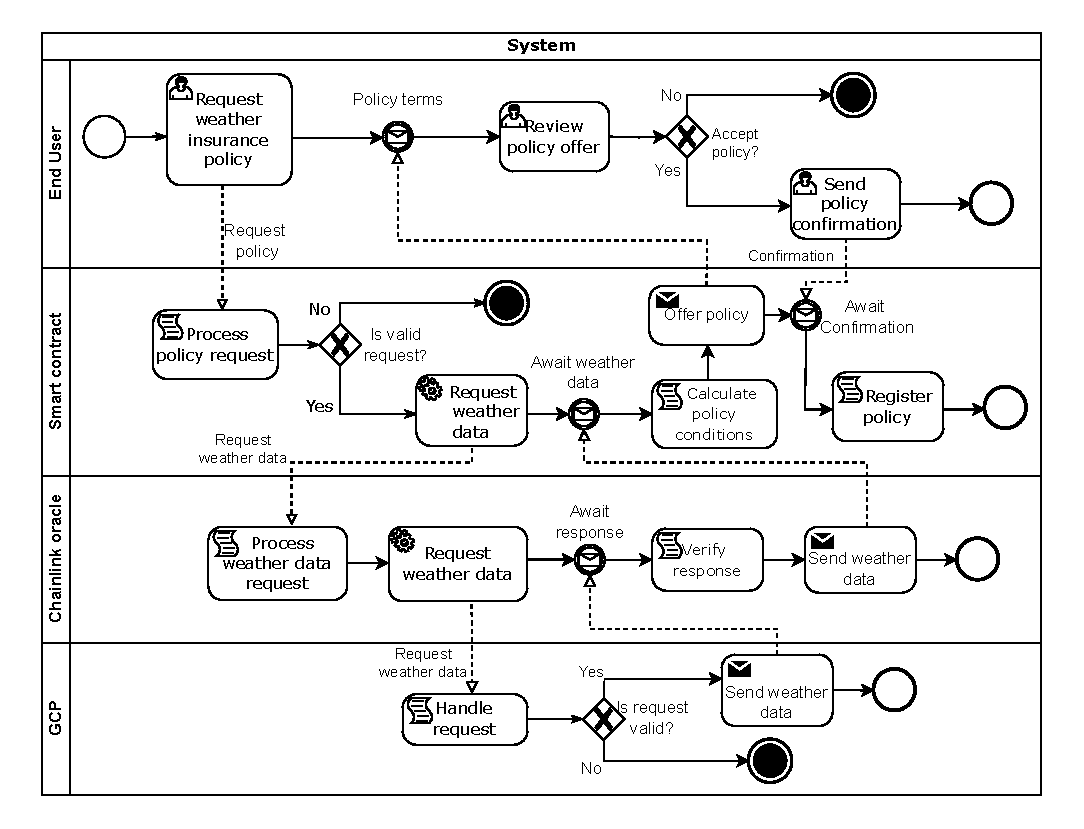
\includegraphics[width=1\textwidth]{figures/flow-purchase-policy.drawio.pdf}
    \caption{Sequence diagram illustrating the process of purchasing an insurance policy in the proposed system. \textit{Source: Author's own representation.}}
    \label{fig:purchasePolicyFlow}
\end{figure}

\begin{table}[ht]
    \centering
    \renewcommand{\arraystretch}{1.3}
\begin{tabular}{|>{\centering\arraybackslash}m{2cm}|>{\centering\arraybackslash}p{5cm}|>{\centering\arraybackslash}m{5cm}|>{\centering\arraybackslash}m{3cm}|}
    \hline
    \textbf{Name} & \textbf{Parameters} & \textbf{Description} & \textbf{Response} \\ 
    \hline
    Request policy & \makecell{Location: String \\ Coverage start date: Date \\ Coverage end date: Date \\ Type of coverage: Enum}  & Requests a policy with the given parameters as the underlying conditions & Binding policy offer including financial conditions and a unique policy ID\\ 
    \hline
    Request weather data & \makecell{Location: String \\ Weather start date: Date \\ Weather end date: Date \\ Type of weather data: Enum \\ Frequency: Enum \\ Data Type: Enum} & Requests weather data in a specific date range. Examples for weather data types are rainfall, wind speed and temperature. Frequency indicates the data granularity (e.g. hourly, daily). Data Type can be either forecast or historical. &  Weather data in JSON format \\ 
    \hline
    Confirmation & \makecell{Policy ID: String \\ Confirmed: Boolean} & Sends a confirmation to the smart contract with the specific policy ID & - \\ 
    \hline
\end{tabular}
    \caption{Requests depicted in \cref{fig:purchasePolicyFlow} and their respective parameters. \textit{Source: Author's own representation.}}
    \label{tab:flowRequests}
\end{table}

The end user starts the process by requesting a weather insurance policy from the smart contract. This interaction happens through the use of a decentralized app (dApp) \cref{subsection:decentralizedApp}, which is not explicitly mentioned in the diagram but can be thought of as the interface enabling the end user to interact directly with the smart contract. Through the dApp, the end user can request a weather insurance policy. In \cref{tab:flowRequests}, we find the detailed description of each request. In the policy request, the user has to specify the conditions of the policy. These include the location, start and end date, the type of coverage (for example, drought coverage or storm coverage), as well as the data type (whether the request should return historical or forecast data).

The smart contract then fetches the necessary weather data needed for the calculation of the policy conditions by sending a request to the Chainlink oracle containing the necessary parameters (see "Weather data request" in \cref{tab:flowRequests}). The Chainlink oracle propagates this request to the Google Cloud Platform (GCP). Due to the decentralized nature of Chainlink oracles, this request is sent multiple times to the GCP from different Chainlink nodes (see \cref{subsection:ChainlinkOracle}). The responses from each of these requests are then analyzed and verified by the Chainlink network before being sent back to the smart contract. The smart contract calculates the policy conditions (such as the premium amount) and sends an offer to the end user. If the end user accepts the terms offered by the smart contract, then the policy is valid and registered on the blockchain.

Note that in the diagram there are two "Request weather data" requests depicted. One is from the smart contract to the Chainlink oracle and one from the Chainlink oracle to the GCP. Even though these requests differ in their technical details (such as type of request and authorization headers), we have combined them in \cref{tab:flowRequests} as one entry. This was chosen specifically for simplicity purposes, since the diagram is an abstraction of a policy purchase process and leaves space for flexibility in technical implementation.

\subsection{Trigger Policy Payout}\label{subsection:policyPayoutTrigger}
The second data flow is shown in \cref{fig:payoutFlow}. It presents the process of triggering a policy payout. This payout happens when the specified policy conditions from \cref{subsection:purchasePolicyFlow} are fulfilled (assuming a policy has been agreed upon between the end user and the smart contract beforehand).

A key decision in the design of the payout process is determining what triggers an eligibility check and the following payout process. A possible solution would be to use scheduled tasks that periodically trigger an eligibility request on every policy held by the smart contract. Since the Ethereum blockchain does not support scheduled or automated tasks natively, such functionality would require an external solution. For example, Chainlink offers an automation service \autocite{chainlink_automation} with which it would be possible to trigger a scheduled eligibility check on the smart contract (for example, once a day). This service would, however, cost gas, which has to be paid by the smart contract and would result in a lot of unnecessary transactions. In our proposed solution, the end user initiates the eligibility check instead. This decision prioritizes simplicity and cost-efficiency, avoiding unnecessary transactions that would otherwise increase the policy premium for the end user.

After the end user has initiated the eligibility check through the use of a decentralized app (dApp), the smart contract gathers the weather data for the specific location and covered duration of the policy. This process of retrieving the relevant weather data is similar to the one in \cref{subsection:purchasePolicyFlow}, with a key distinction being that the weather data contains past data and not forecast data. Once the weather data is received, the smart contract evaluates whether the conditions for a payout are met and communicates the outcome to the end user. If the end user is eligible for a payout, they can submit a request to the smart contract, which will then transfer the agreed-upon funds as specified in the policy.

\begin{figure}[ht]
    \centering
    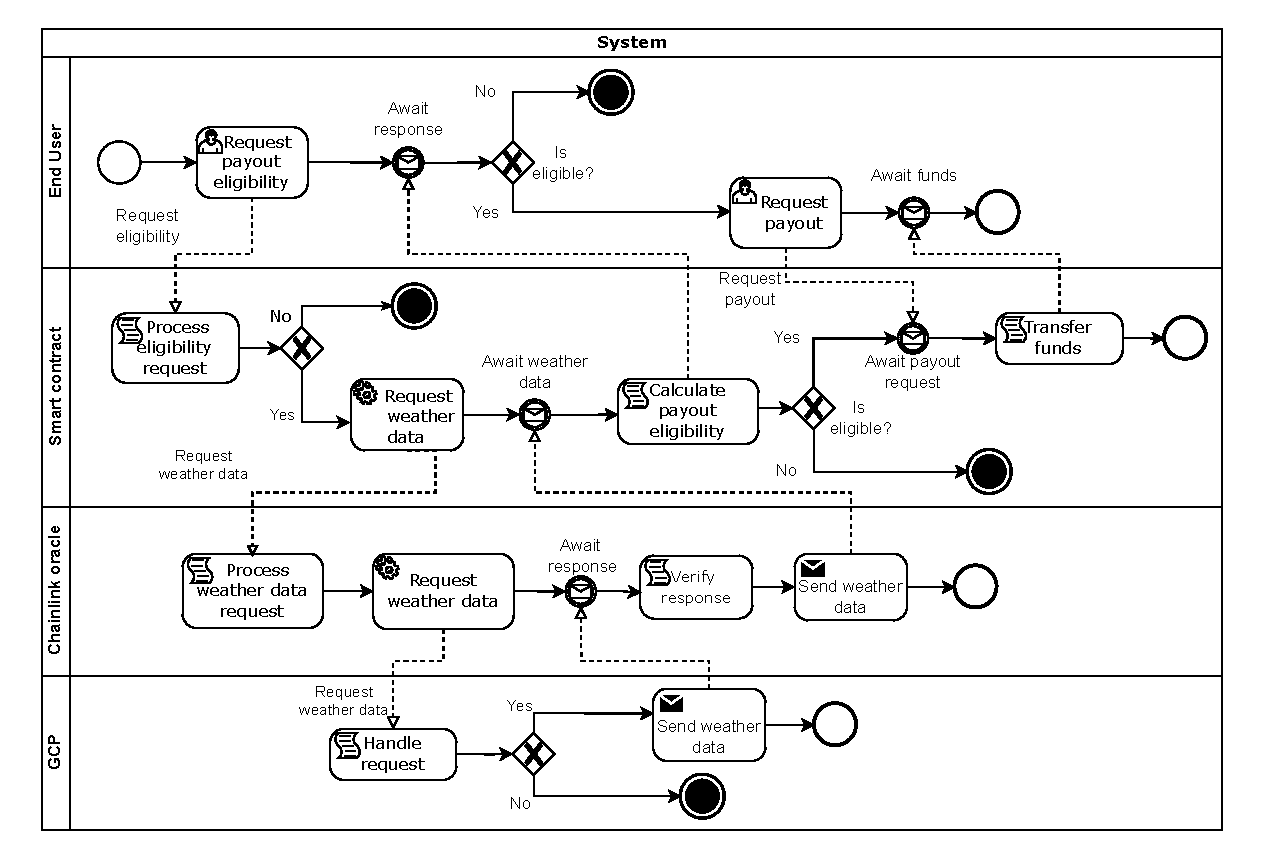
\includegraphics[width=1\textwidth]{figures/flow-policy-payout-trigger.drawio.pdf}
    \caption{Sequence diagram illustrating the process of triggering a policy payout. \textit{Source: Author's own representation.}}
    \label{fig:payoutFlow}
\end{figure}

\begin{table}[ht]
    \centering
    \renewcommand{\arraystretch}{1.3}
\begin{tabular}{|>{\centering\arraybackslash}m{2cm}|>{\centering\arraybackslash}p{5cm}|>{\centering\arraybackslash}m{5cm}|>{\centering\arraybackslash}m{3cm}|}
    \hline
    \textbf{Name} & \textbf{Parameters} & \textbf{Description} & \textbf{Response} \\ 
    \hline
    Request eligibility & \makecell{Policy ID: String}  & Requests an eligibility check, which is then performed by the smart contract. & Whether the policy is eligible for a payout or not in JSON format. \\
    \hline
    Request weather data & \makecell{Location: String \\ Weather start date: Date \\ Weather end date: Date \\ Type of weather data: Enum \\ Frequency: Enum \\ Data Type: Enum} & Requests weather data in a specific date range. Examples of weather data types include rainfall, wind speed, and temperature. Frequency indicates the data granularity (e.g. hourly, daily). Data Type can be either forecast or historical. &  Weather data in JSON format. \\ 
    \hline
    Request payout & \makecell{Policy ID: String} & Requests the payout of funds. & Amount of funds specified in the policy. \\ 
    \hline
\end{tabular}
    \caption{Requests depicted in \cref{fig:payoutFlow} and their respective parameters. \textit{Source: Author's own representation.}}
    \label{tab:payoutFlowRequests}
\end{table}

\subsection{Interaction with the Smart Contract}\label{interaction_with_smartcontract}
As mentioned in \cref{subsection:purchasePolicyFlow} and \cref{subsection:policyPayoutTrigger}, the end user communicates with the smart contract through a decentralized app (see \cref{subsection:decentralizedApp}). The dApp interface is indistinguishable from a regular app interface, with the difference being that it interacts directly with the blockchain instead of a traditional backend. Within the dApp, the end user can create the requests and enter the relevant parameters. Once the user submits a request, the dApp creates a transaction that is signed using the end user's digital wallet. This transaction is then broadcasted to the blockchain, where it can interact directly with the smart contract.

As the focus of this prototype is primarily on the general architecture of a blockchain-based weather insurance solution and its smart contract functionality, we will not dive further into the specifics of decentralized app (dApp) development, since it is not necessary for the subsequent analysis.

\subsection{Calculating Policy Conditions}
One of the core functions of the smart contract is calculating the policy conditions. In \cref{fig:purchasePolicyFlow}, it is presented as an internal process of the smart contract. This process involves assessing the parameters provided by the end user in the "Request policy" request (see \cref{tab:flowRequests}) as well as the weather data that the smart contract receives from GCP through the "Request weather data" request (see \cref{tab:flowRequests}).

In a first validation step, the smart contract ensures that all the parameters are valid, for example, that the location is within a supported region and that the coverage is within the allowed limits. The latter is defined through the furthest available forecast data, which in our solution is 16 days \autocite{NOAA_GFS}. Next, the smart contract calculates the policy conditions based on the following parameters:

\begin{itemize}
    \item Premium amount (the cost of the policy that is paid by the end user)
    \item Trigger conditions (specific thresholds or events that must occur for a payout to be issued, for example rainfall above a certain level)
    \item Coverage limit (the maximum payout amount available under the policy in the case the conditions for a payout are met)
\end{itemize}

Note that the coverage limit is defined by the end user in the "Request policy" request (see \cref{tab:flowRequests}), but it must still be validated and included in the policy by the smart contract, as there may be limits on the maximum coverage amount due to the total funds held by the smart contract.

Calculating the premium amount is the most critical part of the policy conditions. It determines the balance between risk and reward for both the end user and the smart contract. The premium is determined using a formula that considers the following key factors:

\begin{itemize}
    \item Coverage duration
    \item Location
    \item Type of coverage
    \item Forecast weather data
    \item The contract margin
\end{itemize}

This formula represents a fundamental approach to premium calculation. However, it can be further refined by including historical data and actuarial models, allowing for a more dynamic calculation based on real-world risk. Developing a fully-realized mathematical formula suitable for use in a production environment is beyond the scope of this thesis. Instead, we focus on identifying and outlining the key factors included in the formula.

\subsection{Fetching Weather Data}
Both in \cref{fig:purchasePolicyFlow} and in \cref{fig:payoutFlow}, the retrieval of weather data from GCP plays a central role. The security and transparency of our blockchain-based system are only as strong as each component involved in the data retrieval chain. By using Chainlink oracles (see \cref{subsection:ChainlinkOracle}), the smart contract can maintain its decentralized nature.

\section{Real-World Application of the Prototype}\label{section:real_world_application_prototype}
This section explores the practical applications and broader implications of the blockchain-based weather insurance prototype in real-world scenarios. By addressing challenges specific to various industries and sectors, the system shows its ability to improve current insurance practices. Additionally, this section highlights the system's scalability and its ability to reach global audiences, while also acknowledging potential technological and regulatory barriers that need to be addressed for a successful implementation.

\subsection{Application Scenarios}
The following subsections outline three potential real-world applications for our proposed system, presenting how our system's advantages can be effectively leveraged to address specific challenges in each use-case.

\subsubsection{Disaster Relief Efforts}\label{disaster_relief}
Certain regions and countries are particularly vulnerable to extreme weather events and catastrophes, such as floods, hurricanes or droughts. As described in Chapter 1 (see \cref{section:background}), these disasters can result in significant loss of life and extensive financial damage. Relief efforts for such catastrophes are often concentrated in specific areas and rely heavily on government and aid organization support.

By offering transparent weather insurance to governments and humanitarian organizations, the financial burden of disaster relief can be better managed and distributed. As these organizations and governments are often funded through taxpayer money, the proposed application ensures that payouts are automated and verifiable to the general public through blockchain technology, enhancing transparency, trust and accountability in the use of such funds.

\subsubsection{Tourism Industry}\label{tourism_industry}
The tourism industry can be very sensitive to weather conditions, particularly in regions prone to extreme or unexpected weather events, such as heavy rainfall, storms or prolonged droughts. A traveler visiting a region with a high risk of heavy rainfall might want to complete short-term insurance to protect their trip costs in case of such a weather event.

In this application, the system's ability to complete quick policy insurance and automated payouts ensures that the customer can obtain weather insurance on short notice without much bureaucracy involved. This makes the system suitable for spontaneous decisions, which are very common in the tourism sector. Unlike the disaster relief application \cref{disaster_relief}, which focuses on large-scale policies for a few large policyholders, this application is tailored to a smaller-scale, high-volume model.

\subsubsection{Renewable Energy Sector}
Renewable energy projects, such as wind farms, solar parks and hydroelectric plants, are highly dependent on favorable weather conditions. Adverse weather conditions, such as long cloud cover, insufficient wind speeds or droughts can significantly reduce energy output, which can impact the financial stability and operational efficiency of such projects.

The proposed blockchain-based weather insurance system offers a practical solution to mitigate these risks. Through automated payouts when predefined conditions are met, such as insufficient wind speeds or weak sunlight, the system provides project operators with quick financial compensation.

Similar to the disaster relief efforts application \cref{disaster_relief}, large energy projects are often funded by governments. The transparent nature of our blockchain-based system allows the general public to oversee how funds are allocated, used and distributed. This enhances accountability, builds public trust and ensures the funds are managed efficiently and fairly.

\subsection{Scalability and Global Reach}\label{scalability_global_reach}
Unlike traditional insurance systems, which often face bottlenecks due to their reliance on centrally managed infrastructure, the proposed blockchain-based system leverages decentralized technology to simplify policy management, claims processing and payouts. However, achieving wide-range scalability remains a significant challenge. The system's reliance on the Ethereum blockchain introduces limitations due to throughput problems and high gas fees, as mentioned in Chapter 1 (see \cref{technical_challenges_chapter1}). These issues can result in delays and increased costs, particularly as the number of users and transactions grows. While decentralized networks like Chainlink and widely available datasets from GCP offer global applicability, the combination of technical and economic constraints of the Ethereum blockchain limits the efficient scaling of the system to accommodate a large user base across different regions and jurisdictions.

\subsection{Regulatory Barriers of the Prototype}
The regulatory challenges presented in Chapter 1 (see \cref{regulatory_challenges_chapter1}) significantly affect the feasibility of implementing the blockchain-based weather insurance prototype. The lack of universal legal recognition for smart contracts creates uncertainty, especially for applications such as disaster relief and renewable energy, where automated payouts rely on enforceable agreements. If smart contracts are not legally binding, their ability to reduce bureaucracy and ensure efficient operations is greatly diminished if not eliminated.

Compliance with consumer protection and data privacy regulations also poses challenges. Automated transactions may conflict with local laws if users are unable to contest or reverse them. This is particularly problematic in consumer-facing applications like tourism insurance, where disputes over denied payouts can erode trust. Furthermore, the immutable nature of blockchain data storage may conflict with privacy laws, such as the GDPR's "right to be forgotten", limiting the system's applicability in regions with strict data regulations.

Cross-border transactions further complicate the system's scalability. The decentralized architecture relies on interoperability across jurisdictions, each with diffrent requirements for taxation, anti-money laundering (AML) policies and know-your-customer (KYC) compliance. These regulatory differences can introduce inefficiencies and operational complexities, impacting the system's core advantages of transparency, efficiency and trust. Interoperability across borders is also essential for addressing systemic risk described in \cref{systemic_risk}. Without seamless operations, bureaucratic processes across different jurisdictions could reduce the system's perceived efficiency, which limits its ability to scale globally. Coupled with the technical scalability challenges discussed in \cref{scalability_global_reach}, these regulatory barriers further diminish the feasibility of developing a global and scalable solution.
\chapter{Development of the Prototype}\label{chapter:development_prototype}
\section{Requirements}\label{section:requirements}

In order to provide the blockchain-based weather insurance, our system must fulfill several key requirements. In this section we describe each category of requirements in a dedicated subsection.

\subsection{Functional Requirements}\label{subsection:functionalRequirements}

\begin{itemize}
    \item \textbf{User Interaction}
    \begin{itemize}
        \item The system must provide a user interface for purchasing policies and triggering payout eligibility checks. 
    \end{itemize}

    \item \textbf{Weather Data Integration} 
    \begin{itemize}
        \item The system must be able to receive and process global weather data from reliable and trusted external sources such as Global Surface Summary of the Day (GSOD) and Global Forecast System (GFS)
        \item Both historical and forecast data must be available
    \end{itemize}
    
    \item \textbf{Smart Contract}
    \begin{itemize}
        \item The smart contract must allow end users to purchase and terminate weather-based insurance policies based on parameters provided by the end user and the external sources.
        \item The smart contract must store the policy terms.
        \item The smart contract must be able to perform eligibility checks on existing policies.
        \item The smart contract must be able to payout funds for policies that have passed eligibility checks.
    \end{itemize}
    
    \item \textbf{Oracle Integration}
    \begin{itemize}
        \item The system must use Chainlink oracles to retrieve and verify weather data from GCP datasets.
    \end{itemize}
\end{itemize}

\subsection{Non-Functional Requirements}

\begin{enumerate}
    \item \textbf{Security}
    \begin{itemize}
        \item All the bilateral interactions between the smart contract, Chainlink oracles, GCP and the end user must be secure.
    \end{itemize}
    
    \item \textbf{Scalability}
    \begin{itemize}
        \item The system must be able to scale to handle large amounts of policies and end users.
    \end{itemize}
    
    \item \textbf{Transparency}
    \begin{itemize}
        \item All transactions and insurance claims must be recorded on the blockchain for transparency purposes.
    \end{itemize}
\end{enumerate}

\subsection{Technical Requirements}\label{subsection:technicalRequirements}

\begin{enumerate}
    \item \textbf{Blockchain Platform}
    \begin{itemize}
        \item The smart contract must be deployed on the Ethereum blockchain
    \end{itemize}
    
    \item \textbf{Data retrieval}
    \begin{itemize}
        \item The system must be able to retreive weather data from GCP.
    \end{itemize}
    
    \item \textbf{Chainlink Oracle}
    \begin{itemize}
        \item The system must integrate with a Chainlink node to facilitate data retrieval from GCP.
    \end{itemize}
\end{enumerate}

\section{Architecture}

In this section we will propose the architecture for our blockchain-based weather insurance system. First we present a high-level overview of the system and then elaborate on the most important components in a dedicated subsection for each component.

\subsection{General Overview}\label{subsection:generalOverview}

In \cref{fig:generalArchitecture} we present an overview of the general architecture of our proposed system. The center of the architecture is the smart contract deployed on the Ethereum blockchain. It manages all policies and handles the payout process. The end user interacts directly with the smart contract through the use of a decentralized app (see \cref{subsection:decentralizedApp}), where they can request insurance policies and eligibility checks.

The weather data is provided by Global Surface Summary of the Day (GSOD) and Global Forecast System (GFS) respectively. These datasets can be accessed via GCP BigQuery and GCP Storage through the GCP API interface. To bridge the gap between the off-chain data from GCP and the on-chain smart contract, the system uses a Chainlink Oracle (see \cref{subsection:ChainlinkOracle}). This Chainlink Oracle retrieves the weather data from GCP through its API Iiterface and passes it on to the smart contract on the Ethereum blockchain.

This architecture effectively addresses the technical requirements defined in \cref{subsection:technicalRequirements} and ensures compatible and reliable communications between each component.

\begin{figure}[h]
    \centering
    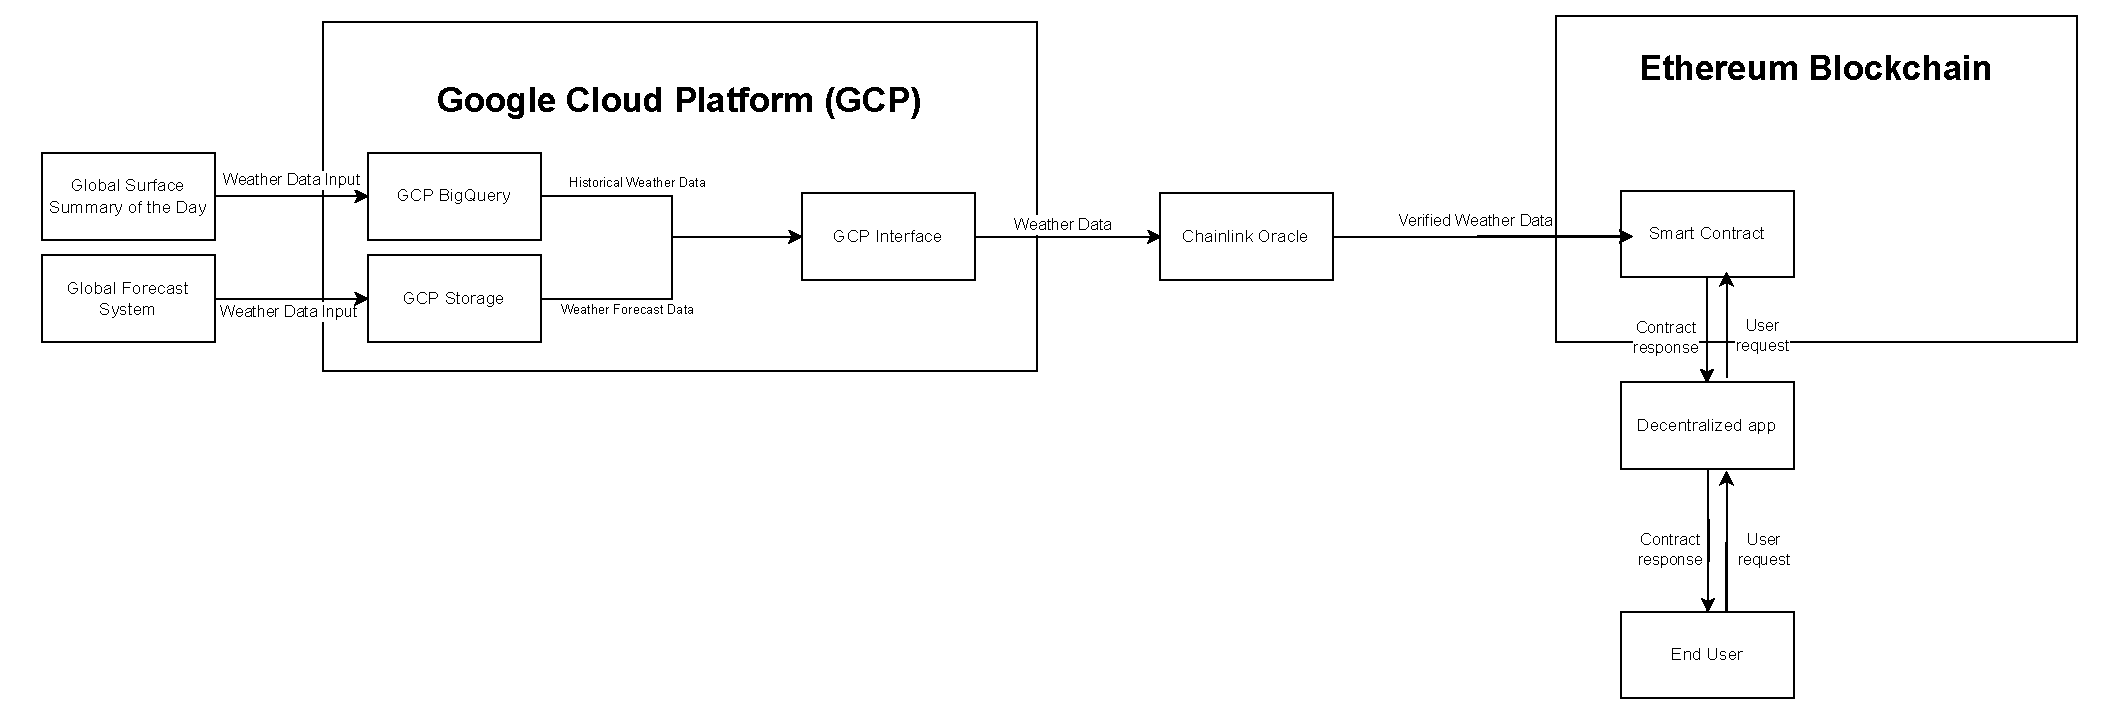
\includegraphics[width=0.95\textwidth]{figures/architecture-overview.drawio.pdf}
    \caption{Diagram showing the architecture of the proposed solution. \textit{Source: Author's own representation.}}
    \label{fig:generalArchitecture}
\end{figure}

\subsection{Decentralized App}\label{subsection:decentralizedApp}

The decentralized application (DApp) allows a non-technical end user to directly interact with the blockchain. Through its interface a user can request insurance policies, eligibility checks and receive payout funds. Unlike traditional applications, which interact with a centrally managed backend, decentralized applications interact directly with a blockchain.

This interaction requires a digital wallet (for example MetaMask) which enables the user to initiate and sign a transaction when making a request, such as purchasing an insurance policy. In our architecture, the dApp serves as the primary interface in order for the end-users to interact with the smart contract. 

\subsection{Integration of Chainlink Oracles and the Google Cloud Platform}\label{subsection:ChainlinkOracle}

Since the weather data from GSOD and GFS, which is accessed through the GCP datasets, is not directly available from the on-chain environment of the smart contract we need to leverage oracles, which retreive and verify external data before delivering it to the blockchain.

In our proposed system, Chainlink oracles are used to securely interact with the GCP and pass the data on to the smart contract. The Chainlink oracle network consists of globally distributed nodes. When a request is triggered, multiple nodes independently access GCP and receive the weather data specified in the request. If any nodes return results that differ from the majority, they are flagged as potentially malicious. This decentralized approach ensures that only verified and reliable weather data is passed on to the smart contract.

\section{Data flow}

In this section, we examine the two primary data flow scenarios central to our blockchain-based weather insurance system: the process of purchasing a weather insurance policy (see \cref{subsection:purchasePolicyFlow}) and the process of triggering a policy payout (see \cref{subsection:policyPayoutTrigger}). These scenarios represent the fundamental interactions between the end user, the smart contract and the external data sources. In the subsequent chapters we elaborate on the core functionalities utilized in the two scenarios such as the process of retreiving weather data and calculating the policy conditions.

\subsection{Purchase Weather Insurance Policy}\label{subsection:purchasePolicyFlow}

The sequence diagram in \cref{fig:purchasePolicyFlow} outlines the steps involved in purchasing a weather insurance policy in our proposed system. The main components are the end user, the smart contract, Chainlink oracle and the Google Cloud Platform (GCP). Each of these components play a central role in enabling the policy purchase and the associated data retrieval and validation processes. Every request between components includes a set of parameters. These parameters contain the necessary information that each component needs in order to perform its role and functions accurately. For example, in a purchase policy request parameters such as location, coverage duration and type of coverage are sent to the smart contract. Table \cref{tab:flowRequests} contains all requests with their respective parameters.

\begin{figure}[h]
    \centering
    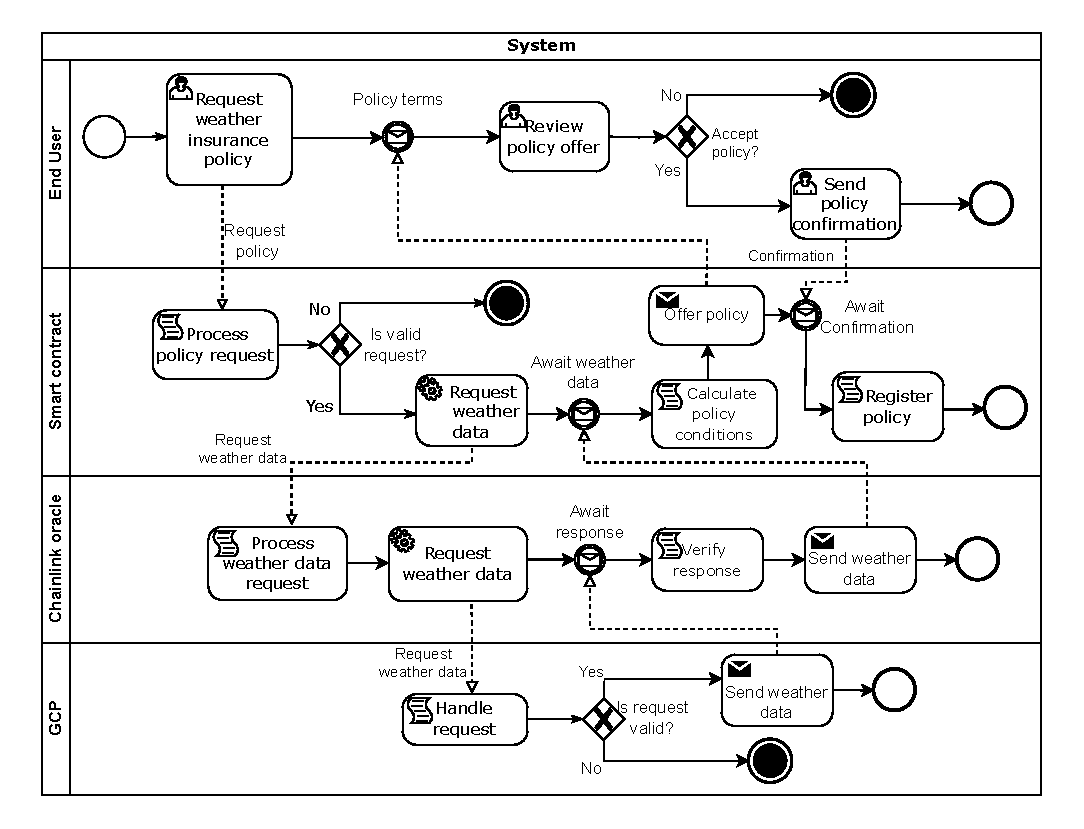
\includegraphics[width=0.95\textwidth]{figures/flow-purchase-policy.drawio.pdf}
    \caption{Sequence diagram of purchasing an insurance policy in our proposed system \textit{Source: Author's own representation.}}
    \label{fig:purchasePolicyFlow}
\end{figure}

\begin{table}[h]
    \centering
    \renewcommand{\arraystretch}{1.3}
\begin{tabular}{|>{\centering\arraybackslash}m{2cm}|>{\centering\arraybackslash}p{5cm}|>{\centering\arraybackslash}m{5cm}|>{\centering\arraybackslash}m{3cm}|}
    \hline
    \textbf{Name} & \textbf{Parameters} & \textbf{Description} & \textbf{Response} \\ 
    \hline
    Request policy & \makecell{Location: String \\ Coverage start date: Date \\ Coverage end date: Date \\ Type of coverage: Enum}  & Requests a policy with the given parameters as the underlying conditions & Binding policy offer including financial conditions and a unique policy ID\\ 
    \hline
    Request weather data & \makecell{Location: String \\ Weather start date: Date \\ Weather end date: Date \\ Type of weather data: Enum \\ Frequency: Enum \\ Data Type: Enum} & Requests weather data in a specific date range. Examples for weather data types are rainfall, wind speed and temperature. Frequency indicates the data granularity (e.g. hourly, daily). Data Type can be either forecast or historical. &  Weather data in JSON format \\ 
    \hline
    Confirmation & \makecell{Policy ID: String \\ Confirmed: Boolean} & Sends a confirmation to the smart contract with the specific policy ID & - \\ 
    \hline
\end{tabular}
    \caption{Requests in \cref{fig:purchasePolicyFlow} with their parameters \textit{Source: Author's own representation.}}
    \label{tab:flowRequests}
\end{table}

The end user starts the process by requesting a weather insurance policy from the smart contract. This interaction happens through the use of a decentralized app (dApp) \cref{subsection:decentralizedApp}, which is not explicitly mentioned in the diagram but can be thought of as the interface enabling the end user to interact directly with the smart contract. Through the dApp the end user can request a weather insurance policy. In table \cref{tab:flowRequests} we find the detailed description of each request. In the policy request the user has to specify the conditions of the policy, these include the location, start- and end-date, the type of coverage (for example drought coverage or storm coverage) as well as the data type (whether the request should return historical or forecast data).

The smart contract then fetches the necessary weather data needed for the calculation of the policy conditions by sending a request to the Chainlink oracle containing the necessary parameters (see "Weather data request" in table \cref{tab:flowRequests}). The Chainlink oracle propagates this request to the Google Cloud Platform (GCP). Due to the decentralized nature of Chainlink oracles this request is sent multiple times to the GCP from different Chainlink nodes (see \cref{subsection:ChainlinkOracle}). The responses from each of these requests are then analyzed and verified by the Chainlink network beofre being sent back to the smart contract. The smart contract calculates the policy conditions (such as the premium amount) and sends an offer to the end user. If the end user accepts the terms offered by the smart contract, then the policy is valid and registered on the blockchain.

Note that in the diagram there are two "Request weather data" requests depicted. One is from the smart contract to the Chainlink oracle and one from the Chainlink oracle to the GCP. Even though these requests differ in their technical details (such as type of request and authorization headers) we have combined them in table \cref{tab:flowRequests} as one entry. This was chosen specifically for simplicity purposes, since the diagram is an abstraction of a policy purchase process and leaves space for flexibility in technical implementation.

\subsection{Trigger Policy Payout}\label{subsection:policyPayoutTrigger}

The second data flow is shown in \cref{fig:payoutFlow}. It presents the process of triggering a policy payout. This payout happens when the specified policy conditions from \cref{subsection:purchasePolicyFlow} are fulfilled (assuming a policy has been agreed upon between the end user and the smart contract beforehand). 

A key decision in the design of the payout process is determining is what triggers an eligibility check and the following payout process. A possible solution would be to use scheduled tasks that periodically trigger an eligibility request on every policy held by the smart contract. Since the Ethereum blockchain does not support scheduled or automated tasks natively, such a solution would require an external solution. For example Chainlink offers an automation service \autocite{chainlink_automation} with which it would be possible to trigger a scheduled eligibility check on the smart contract (for example once a day). This service would however cost gas which has to be paid by the smart contract and result in a lot of unnecessary transactions. In our proposed solution, the end user initiates the eligibility check instead. This decision prioritizes simplicity and cost-efficiency, avoiding unnecessary transactions that would otherwise increase the policy premium for the end user.

After the end user has initiated the eligibility check through the use of a decentralized App (dApp), the smart contract gathers the weather data for the specific location and covered duration of the policy. This process of retrieving the relevant weather data is similar to the one in \cref{subsection:purchasePolicyFlow}, with a key distinciton being that the weather data contains past data and not forecast data. Once the weather data is received, the smart contract evaluates whether the conditions for a payout are met and communicates the outcome to the end user. If the end user is eligible for a payout, they can submit a request to the smart contract, which will then transfer the agreed-upon funds as specified in the policy.


\begin{figure}[h]
    \centering
    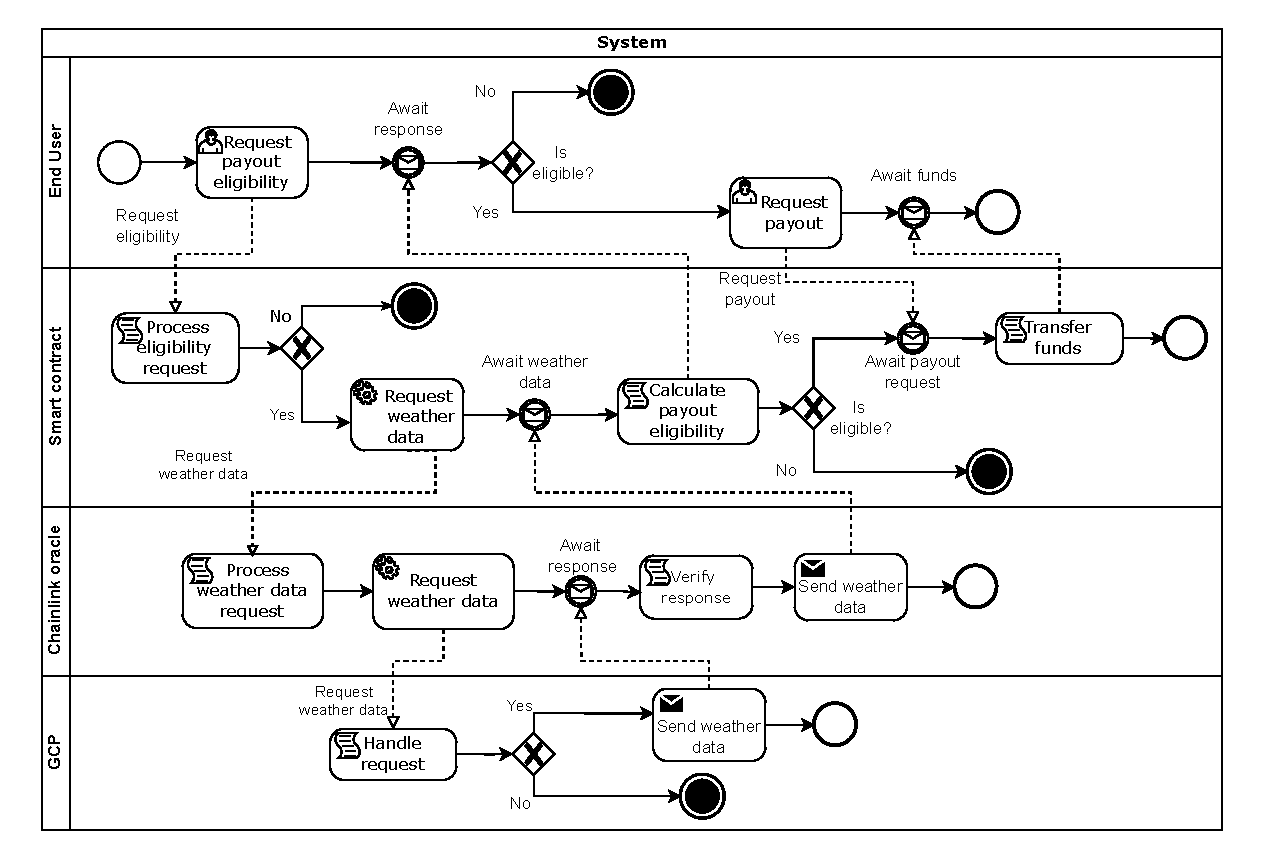
\includegraphics[width=0.95\textwidth]{figures/flow-policy-payout-trigger.drawio.pdf}
    \caption{Sequence diagram of triggering a policy payout \textit{Source: Author's own representation.}}
    \label{fig:payoutFlow}
\end{figure}

\begin{table}[h]
    \centering
    \renewcommand{\arraystretch}{1.3}
\begin{tabular}{|>{\centering\arraybackslash}m{2cm}|>{\centering\arraybackslash}p{5cm}|>{\centering\arraybackslash}m{5cm}|>{\centering\arraybackslash}m{3cm}|}
    \hline
    \textbf{Name} & \textbf{Parameters} & \textbf{Description} & \textbf{Response} \\ 
    \hline
    Request eligibility & \makecell{Policy ID: String}  & Requests an eligibility check, which is then performed by the smart contract. & Whether the policy is eligible for a payout or not in JSON format. \\
    \hline
    Request weather data & \makecell{Location: String \\ Weather start date: Date \\ Weather end date: Date \\ Type of weather data: Enum \\ Frequency: Enum \\ Data Type: Enum} & Requests weather data in a specific date range. Examples of weather data types include rainfall, wind speed, and temperature. Frequency indicates the data granularity (e.g. hourly, daily). Data Type can be either forecast or historical. &  Weather data in JSON format. \\ 
    \hline
    Request payout & \makecell{Policy ID: String} & Requests the payout of funds. & Amount of funds specified in the policy. \\ 
    \hline
\end{tabular}
    \caption{Requests \cref{fig:payoutFlow} with their respective parameters \textit{Source: Author's own representation.}}
    \label{tab:payoutFlowRequests}
\end{table}

\subsection{Interaction with the Smart Contract}

As mentioned in \cref{subsection:purchasePolicyFlow} and \cref{subsection:policyPayoutTrigger}, the end user communicates with the smart contract through a decentralized app (see \cref{subsection:decentralizedApp}). The dApp interface is indistinguishable from a regular app interface, with the difference being that it interacts directly with the blockchain instead of a traditional backend. Within the dApp the end user can create the requests and enter the relevant parameters. Once the user submits a request, the dApp creates a transaction that is signed using the end user's digital wallet. This transaction is then broadcasted to the blockchain, where it can interact directly with the smart contract.

As the focus of this prototype is primarily on the general architecture of a blockchain-based weather insurance solution and its smart contract functionality, we will not delve further into the specifics of decentralized app (dApp) development, since it is not necessary for the subsequent analysis.

\subsection{Calculating Policy Conditions}

One of the core functions of the smart contract is calculating the policy conditions. In \cref{fig:purchasePolicyFlow} it is presented as an internal process of the smart contract. This process involves assessing the parameters provided by the end user in the "Request policy" request (see \cref{tab:flowRequests}) as well as the weather data that the smart contract receives from GCP through the "Request weather data" request (see \cref{tab:flowRequests}).

In a first validation step, the smart contract ensures that all the parameters are valid, for example that the location is within a supported region and that the coverage is within the allowed limits. Latter is defined through the furtherst available forecast data, which in our solution is 16 days \autocite{NOAA_GFS}. Next follows the calculation for the policy conditions based on these parameters. These conditions are the following:

\begin{itemize}
    \item Premium amount (the cost of the policy that is paid by the end user)
    \item Trigger conditions (specific thresholds or events that must occur for a payout to be issued, for example rainfall above a certain level)
    \item Coverage limit (the maximum payout amount available under the policy in the case where the conditions for a payout are met)
\end{itemize}

Note that the coverage limit is defined by the end used in the "Request policy" request (see \cref{tab:flowRequests}) but still has to be validated and included in the policy by the smart contract since there may be limits for a maximum coverage amount due to the total funds held by the smart contract.

Calculating the premium amount is the most critical part in the policy conditions. It defines the balance between risk and reward for both the end user and the smart contract. The premium is determined using a formula that considers the following key factors:

\begin{itemize}
    \item Coverage duration
    \item Location
    \item Type of coverage
    \item Forecast weather data
    \item The contract margin
\end{itemize}

This formula represents a fundamental approach for premium calculation. However, it can be further refined by including historical data and actuarial models, allowing for a more dynamic calculation based on real-world risk. Developing a fully-realized mathematical formula suitable for the usage in a production environment is beyond the scope of this thesis. Instead, we focus on identifying and outlining the key factors that are included in the formula. In the analysis chapter (include reference), these factors will be evaluated to compare the premium calculation approach in a blockchain-based insurance system with that of a traditional weather insurance model.

\subsection{Smart contract fetching weather data}

Both in \cref{fig:purchasePolicyFlow} and in \cref{fig:payoutFlow} the retrieval of weather data from GCP plays a central role. The security and transparency of our blockchain-based system is only as strong as each component involved in the data retrieval chain. By using Chainlink oracle (include reference), the smart contract can maintain its decentralized nature. 
\chapter{Analysis and Discussion}\label{chapter:analysis_discussion}
\section{Technological and regulatory barriers of the prototype}\label{section:technological_regulatory_barriers}
\section{Real-world application of the prototype}\label{section:real_world_application_prototype}
\section{Analysis of smart contracts in the insurance industry}\label{section:analysis_smart_contracts_insurance}

\chapter{Summary and Conclusion}\label{chapter:summary_conclusion}
\section{Summary of findings}\label{section:summary_findings}
\section{Conclusions}\label{section:conclusions}
\section{Future work}\label{section:future_work}


\newpage

\appendix
\noappendicestocpagenum
\addappheadtotoc
\appendixpage

\renewcommand{\theequation}{A.\arabic{equation}}

\chapter{Appendix title 1}\label{appendix:title1}

Test appendix 1

%\chapter{Appendix title2}\label{appendix:title2}

Test Appendix 2

\printbibliography

\newpage
\thispagestyle{firststyle}
\section*{Eidesstattliche Erklärung}
Der/Die Verfasser/in erklärt an Eides statt, dass er/sie die vorliegende Arbeit selbständig, ohne fremde Hilfe und ohne Benutzung anderer als die angegebenen Hilfsmittel angefertigt hat. Die aus fremden Quellen (einschliesslich elektronischer Quellen) direkt oder indirekt übernommenen Gedanken sind ausnahmslos als solche kenntlich gemacht. Die Arbeit ist in gleicher oder ähnlicher Form oder auszugsweise im Rahmen einer anderen Prüfung noch nicht vorgelegt worden.\\[2cm]
\dotbox{Ort, Datum} \hfill \dotbox{Unterschrift des/der Verfassers/in}
\end{document}
